%%% Template for AUTHOR's DRAFT paper in FCAA, WITHOUT Journal's head  %%%%%%%%%%%%%%%%%%%%%%%%%%%%%%%%%
%%% by V. Kiryakova, updated Nov. 1, 2014
%%% uses "fcaa.cls", or "fcaa-var.cls" as modifications of "amsart.cls" for the FCAA format,
%%% and auxiliary file "fcaa_style.tex" fixing page margins, fontsize, defs for theorems, proofs etc.
%%% Put the files "fcaa.cls", "fcaa-var.cls" and "fcaa_style.tex" in same directory you prepare the paper

  %\documentclass[twoside,reqno,11pt]{fcaa}  %%% or in case of problems, use as below: %
   \documentclass[twoside,reqno,11pt]{fcaa-var} %

 \input fcaa_style

%%%%%%%%%%%%%%%%%%%%
 \usepackage{hyperref} % Editor will use to create hyperlinks %
% \newcommand{\ord}[2]{\operatorname{ord}_{#2}\left(#1\right)}
 %\newcommand{\deg}{\operatorname{deg}}
% \DeclareMathOperator{\deg}{deg}
 %%% but if the author has problems with the above style file,
 %%% then comment the line \usepackage{hyperref} or replace by this below:
 % \usepackage{upref}
%%%%%%%%%%%%%%%%%%%%
\captionsetup[subfigure]{labelfont=rm}
% to have 2-digits numbering for equation, use:
 \def\theequation{\arabic{section}.\arabic{equation}}

%%%%%%  First page footnote for Copyright and Springer logo
 \def\themycopyrightfootnote{\vspace*{3pt}
 \copyright \, Year\,  Diogenes  Co., Sofia
   \par  \noindent pp. xxx--xxx, DOI: ......................
   \hfill  \vspace*{-36pt}
    %\mbox{\includegraphics[scale=0.65]{DeGryuter.eps}}
  }
%%%%%%%%%%%%%%%%%%%%%%%%%%%%%%%%%%%%%%%%%%%%%%%%%%%%%%%%%%%%
\setcounter{page}{1}
\thispagestyle{empty}
 %%%%%%%%%%%%%%% begin make title %%%%%%%%%%%%%%%%%%%%%%%%%%%%%
 %%% TITLE: texts in [.] is abbreviated (1st line) title for running heads
 %%% Author(s): put in brackets [.] the short author's name

 \title[Fractional-Order Controllers for IS]{fractional-order Controllers  \\ [3pt] for Irrational Systems}
 \author[\normalsize Guel-Cortez et al.]{\normalsize A.-J.\ Guel-Cortez $^1$, Eun-jin Kim $^2$, C.-F. M\'{e}ndez-Barrios$^3$, Mihir Sen$^4$}

 %%% obligatory give the full and abbreviated authors' names %%%
 %%%%%%%%%%%%%%%%%%%%%%%%%%%%%%%%%%%%%%%%%%%%%%%%%%%%%%%%%%%%%%%
                    % THE BEGINNING %
 \begin{document}

 \vbox to 2.5cm { \vfill }

%%% to make empty space of approx. 2.5cm %%%%%%
%%% will be replaced by Editor with the journal's and publoishers logos %%%%%%%%

 \bigskip \medskip

%%%% Abstract %%%%%%%%%%%%%%%%%%%%%%%%%
 \begin{abstract}
 	In this contribution, we investigate fractional-order controllers of the type $PD^\mu$ and $PI^\lambda$ applied to a class of irrational transfer function models that appear in large-scale systems, such as, networks of mechanical or electrical elements and distributed parameter systems. More precisely, we consider the controller $k_p+k_\eta s^\alpha$ in the Laplace domain with $-1\leq\alpha\leq1$ and present the stability analysis in the parameter-space $(k_p,k_\eta,\alpha)$. We further show details of the controller fragility analysis in the parameter plane $(k_p,k_\eta,\alpha)$ as a measurement of the controller robustness. Finally, several specific applications are discussed to demonstrate the utility of our results. %$\deg$

 \medskip

{\it MSC 2010\/}: Primary 93D15; Secondary 26A33, 58E25 ,70Q05

 \smallskip

{\it Key Words and Phrases}: fractional-order controllers, irrational systems, stability analysis, controller's design

 \end{abstract}

 \maketitle

%%%%%%% end make title %%%%%%%%%%%%%%%%%%%%%%%%%%%%%%%%%%
 \vspace*{-16pt}

%%%%%%%% begin papers' body %%%%%%%%%%%%%%%%%%%%%%%%%%%%%

%%%%%%%%%%%%%%%%%%%%%%%%%%% Section 1 %%%%%%%%%%%%%
%\section{Introduction}\label{Sec:1}
\section{Introduction}\label{sec:1}
An irrational system (IS) is a class of system whose model is represented by a transfer function containing irrational orders. In \cite{Sen2018,Mayes2011}, ISs are described as implicit operators because they are solutions to an operator equation. Besides,\cite{Montseny1998} presents ISs as a type of pseudo-differential time-operators whose representation in time domain is diffusive (for further details about the diffusive representation, see \cite{Casenave2010}). 
Examples of ISs can be found in various previous works across different disciplines. For instance, \cite{Mayes2011} introduces an IS model to represent the total operator describing the potential-driven flow dynamics in a large-scale self-similar tree network. In references \cite{Goodwine2018,Leyden2016}, a version with springs and dampers of this IS is examined in order to propose model reductions to robotic formations or cyber-physical systems. In addition, its time response is studied in \cite{Guel-Cortez2018b} with the purpose to analyse the model's feasibility to approximate the time response of large-scale systems. \par 
On the other hand, infinite ladder networks can also be modelled by using an IS representation (for further details, see \cite{Sen2018}). In his famous text \cite{Feynman2006}, Richard Feynman studies an infinite $LC$ ladder circuit and proposes an expression for its total impedance in the form of an IS. Such a model has caused several questions regarding its convergence (for instance, see \cite{Klimo_2016} and the references therein). In \cite{Leyden2018a}, an IS model for an infinite ladder of mass-springs and dampers is introduced toward the goal of efficient modelling complex networks of mechanical systems. Furthermore, in order to describe the power law behaviour in soft tissue, a hierarchical fractal ladder network model is proposed in \cite{Kelly2009}. This model leads to an IS which was approximated by a fractional-order system. Therefore, fractional-order systems can be seen as a special case of ISs. Finally, ISs can also be found when solving partial differential equations or when modelling distributed parameter systems (for further details, see \cite{Curtain1992,Curtain1995,Hernandez2013,Wu2007}). \par 
Since ISs are used as an approximation or model reduction for modelling large-scale complex systems, their stability and control analysis are of great interest for practical applications. In addition, due to the connection of ISs with fractional-order systems, fractional-order controllers may be a suitable option to control ISs. \par 
In recent years, the fractional-order version $PI^\lambda D^\mu$ of the classical $PID$ controller has become popular due to the explosion of fractional calculus applications (see \cite{Shah2016,Tepljakov2013,Guel-Cortez2018,Guel-Cortez2019}). These $PI^\lambda D^\mu$ controllers include a derivative $D^\mu$ and an integral $I^\lambda$ of non-integer orders $\mu>0,\lambda<0\in\R$. The values $\mu$ and $\lambda$ add more degrees of freedom to the controller which creates a more flexible controller in comparison with the classical $PID$ controllers \cite{valerio2013anintroduction}. Moreover, they have been shown to tend good results when applied to fractional-order systems (see \cite{Caponetto2010,Monje2010,Tavazoei2012,Guel-Cortez2018,Guel-Cortez2019}).\par Fractional-$PID$ controllers design has been already studied for different type of systems (for some examples, see \cite{Guel-Cortez2018,Guel-Cortez2019,Petras2019,GHORBANI20199302,Gao2019,Birs2019}). Previously, in \cite{Guel-Cortez2019a} we have introduced the control design of fractional $PD^\mu$ controllers for ISs without analysing the effects of changing the controller's parameter $\mu$ on the stability $(k_p,k_\eta,\mu)$ parameter-space. \par
Another important aspect to consider when designing any type of controllers corresponds to the fragility analysis. Roughly speaking, a controller for which the closed-loop system is destabilized by small perturbations in the controller parameters is called “fragile” \cite{mendez2008fragility}. There are various reasons to study the controller's fragility. Firstly, every controller implementation is subject to the imprecision inherent in analog-digital and digital-analog conversion, finite word length, and finite resolution measuring instruments and round-off errors in numerical computations. Secondly, every paper design requires readjustment because no scalar index can capture all the performance requirements of a control system. \cite{keel1997robust,alfaro2007pid,ho2000non}.\par 

With the above background as motivation, the aim of this paper is to present a procedure to design non-fragile stabilising fractional-order controllers of $PD^\mu$ and $PI^\lambda-$type to a kind of ISs. Such an analysis has been performed by means  the $\mathcal{D}-$composition method \cite{gryazina2008d,gryazina2004d} to obtain the parameter-space $(k_p,k_\eta,\alpha)$, where $k_p,k_d$ and $\alpha$ represent the control parameters that Bounded-Input, Bounded-Output (BIBO) stabilise the IS and by computing the controller's fragility in the parameter-space $(k_p,k_\eta,\alpha)$.\par 
The paper is organised as follows. In Section \ref{sec:Prel}, we revise fundamental concepts and preliminary results that will be used throughout the paper and formulate the main problems to be solved. In Section \ref{sec:main}, we present our controller restrictions and the results on the characterization of the stability crossing boundaries, crossing directions and fragility analysis to solve our described problems. In Section \ref{sec:Numerics}, we analyse several specific examples to show the effectiveness and applicability of the theory. Finally, Section \ref{sec:Concl}, contains some concluding remarks.\par  
The notation used through the paper is as follows: $\mathbb{C}$ is the set of complex numbers, $\bm{i}:=\sqrt{-1}$, all points in the complex plane whose real part are positive, will be called the right half-plane (RHP), whereas all points whose real part are negative will be called the left half-plane (LHP). $\mathbb{C}_+$ and $\mathbb{C}_-$ stand for the closed right half-plane (RHP) and the open RHP of the first Riemann sheet, respectively. Also, for $z \in \C$, $\bar{z}$, $\arg{z}$, $\Re(z)$ and $\Im(z)$ define the complex conjugate, main argument (i.e., $\arg{z}\in(-\pi,\pi]$), and the real and imaginary parts of $z$ respectively. $\R$ ($\R_+$ and $\R_-$) denotes the set of real numbers (strictly positive, strictly negative) and $\N$ and $\Q$ denote the set of natural and rational numbers respectively. For $\bm{x},\bm{y}$ $\in {\C}^n$, the scalar product is denoted by $\langle\bm{x},\bm{y}\rangle=\bm{y}^T\bm{x}$, where $\bm{y}^T$ is the complex conjugate transpose of $\bm{y}$. 

\setcounter{section}{1}
\setcounter{equation}{0}\setcounter{theorem}{0}


\section{Preliminary Results and Problem Formulation}\label{sec:Prel}
In this section, we will review some fundamental definitions and preliminary results that will be useful in the remaining part of the paper.
\begin{definition}[Branch Point, Branch Cut \cite{Cohen2007,Needham1997}]
	A Branch Point (BP) is a point such that the function is discontinuous when going around an arbitrarily small circuit around this point. A Branch Cut (BC) is the union of two BPs by an arbitrary arc (see Fig. \ref{contour1}). This BC connects different sheets of a Riemann-surface.
\end{definition}
%\begin{definition}[The inversion formula \cite{Cohen2007,Thomson1950}]
%In complex analysis, and irrational transfer function like \eqref{sys1} or any linear fractional order system transfer function is considered as a \textit{multivalued function}. For computing the response of such type of systems we can use the Inverse Laplace transform (ILT), but we have to consider the location of its Branch Points (BP) and Branch Cuts (BC) in addition to common singularities like poles. To obtain the ILT of any multivalued function, we use the common inversion formula given by
%\begin{equation}
%f(t)=\tfrac{1}{j2\pi}\int_{\gamma-j\infty}^{\gamma+j\infty}F(s)e^{st}ds=\tfrac{1}{j2\pi}\int_{\textbf{Br}}F(s)e^{st}ds, \label{eqinversion}
%\end{equation}
%where $\textbf{Br}$ stands for the path $\gamma-j\infty$ to $\gamma+j\infty$ with $\gamma\in\mathbb{R}$ to the right of all singularities of $F(s)$, known as \textit{Bromwich path} considered in the region of convergence. 
%\end{definition}
\begin{figure}[h!]
	\centering
	 \input{intc.tex}
	\caption{Integration contour for system \eqref{sys1}.}\label{contour1}
\end{figure}
\begin{theorem}[from \cite{Merrikh-Bayat2008}] \label{th:th1}
	A given multi-valued transfer function is stable if and only if it has no poles in $\mathbb{C}_+$ and no BPs in $\mathbb{C}_-$.
\end{theorem}

\subsection{Problem Formulation}
Consider the multi-valued transfer function of the form
\begin{eqnarray}
% G(s)&=&\frac{N(s)+P(s)}{D(s)+Q(s)}, \label{sys1}
G(s)&=&\frac{N(s)+\sqrt{P(s)}}{D(s)+\sqrt{Q(s)}}, \label{sys1}
\end{eqnarray}
where $N(s)=\sum_{k=0}^{m}b_ks^k,$ $D(s)=\sum_{k=0}^{n}a_ks^k$, $a_i$, $b_i$, $a_n\neq0$ are arbitrary real numbers, and $n\geq m$. Besides, $P(s)$ and $Q(s)$ are second order polinomials with positive real coefficients defined as $P(s)=\beta_2s^2+\beta_1 s+\beta_0$ and $Q(s)=\alpha_2s^2+\alpha_1 s+\alpha_0$, respectively.\\
In the rest of the paper, we will consider that system \eqref{sys1} is constrained by the following assumptions:
\begin{assumption}\label{Assum1}
	Polynomials $N(s)$ and $D(s)$ satisfy the following conditions:
	\begin{itemize}
		\item [(i)] $N(s)$ and $D(s)$ are coprime polynomials.
		\item [(ii)] $|N(\bm{i}\omega)|>0$, $\forall\omega\in\R$.
		\item [(iii)] if $D(\bm{i}\omega^*)=0$, then $|D^\prime(\bm{i}\omega^*)|>0$ with $\omega^*\in\R$.
	\end{itemize}
\end{assumption}
\begin{assumption}\label{Assum2}
	The functions $P(s)$ and $Q(s)$ satisfy the following conditions:
	\begin{itemize}
		\item  [(i)] $\deg Q(s) \geq \deg P(s)$.
		%    \item [(ii)] $\alpha_2\neq a_n$ if $n=2$.
		%\item [(ii)] $Q^2(s_1)=0$ and $P^2(s_2)=0$ $\iff$ $s_1,s_2\notin$ RHP. 
		\item [(iii)] if $\deg(D(s))=\deg(N(s))$, then $\deg Q(s) > \deg P(s)$.
	\end{itemize}
\end{assumption}
Assumption \ref{Assum1} permits us to avoid multiple poles on the imaginary axis. It also prevents $D(s)$ and $N(s)$ from having the same roots and allow us to have a strictly proper transfer function even in the case when $\deg Q(s)=\deg P(s)=0$. On the other hand, Assumption \ref{Assum2} defines rules for the degrees of $P(s),Q(s)$ to obtain a proper transfer function in the case  $\deg N(s)=\deg D(s)=0$ and avoids BPs in the RHP to satisfy the stability requirements of Theorem \ref{th:th1}. The BPs of system \eqref{sys1} are given by the roots $r_{1,P(s)},r_{2,P(s)}$ and $r_{1,Q(s)},r_{2,Q(s)}$ of $P(s)$ and $Q(s)$, respectively. These BPs form the BCs of system \eqref{sys1} as depicted in Fig. \ref{contour1}.\par
Given the assumptions above, the problems of our interest are as follows:
\begin{problem}
	Derive conditions on the parameters $(k_p,k_\eta,\alpha)$ such that the fractional-order controller:
	\begin{equation}
	C(s)=k_p+k_\eta s^\alpha, \label{eqcontrol}
	\end{equation}
	BIBO-stabilizes the closed-loop plant. Fig.~\ref{GCDiagram} describes the closed-loop configuration.% transfer function in Eq.~\eqref{sys1}.
	\begin{figure} %Ambiente ?figure?
		\centering %imagen sin escalar
		\begin{adjustbox}{max width=\columnwidth}


\tikzset{every picture/.style={line width=0.75pt}} %set default line width to 0.75pt        

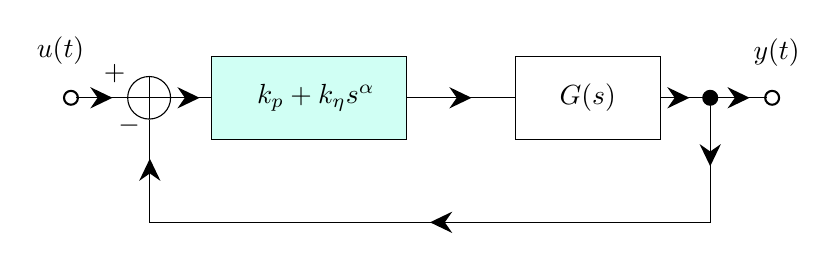
\begin{tikzpicture}[x=0.75pt,y=0.75pt,yscale=-1,xscale=1]
%uncomment if require: \path (0,145.3333282470703); %set diagram left start at 0, and has height of 145.3333282470703

%Shape: Rectangle [id:dp8081499781514234] 
\draw  [fill={rgb, 255:red, 208; green, 255; blue, 244 }  ,fill opacity=1 ] (149.83,31) -- (243.83,31) -- (243.83,71) -- (149.83,71) -- cycle ;
%Shape: Rectangle [id:dp5281027237826732] 
\draw   (296,31) -- (366,31) -- (366,71) -- (296,71) -- cycle ;
%Straight Lines [id:da614101386826865] 
\draw    (244,51) -- (295.83,51) ;


%Straight Lines [id:da8620710599324111] 
\draw    (130,51) -- (149.83,51) ;


%Straight Lines [id:da6418152913677391] 
\draw    (84.35,51) -- (109.33,51) ;

\draw [shift={(82,51)}, rotate = 0] [color={rgb, 255:red, 0; green, 0; blue, 0 }  ][line width=0.75]      (0, 0) circle [x radius= 3.35, y radius= 3.35]   ;
%Straight Lines [id:da25553501722793825] 
\draw    (390,51) -- (417.48,51) ;
\draw [shift={(419.83,51)}, rotate = 0] [color={rgb, 255:red, 0; green, 0; blue, 0 }  ][line width=0.75]      (0, 0) circle [x radius= 3.35, y radius= 3.35]   ;

%Straight Lines [id:da34864449125788677] 
\draw    (390,51) -- (390,111) -- (120,111) -- (120,61.67) ;

\draw [shift={(390,51)}, rotate = 90] [color={rgb, 255:red, 0; green, 0; blue, 0 }  ][fill={rgb, 255:red, 0; green, 0; blue, 0 }  ][line width=0.75]      (0, 0) circle [x radius= 3.35, y radius= 3.35]   ;
%Straight Lines [id:da2457539278941714] 
\draw    (366,51) -- (390,51) ;


%Straight Lines [id:da875448509729424] 
\draw    (102,51) ;
\draw [shift={(102,51)}, rotate = 180] [fill={rgb, 255:red, 0; green, 0; blue, 0 }  ][line width=0.75]  [draw opacity=0] (10.72,-5.15) -- (0,0) -- (10.72,5.15) -- (7.12,0) -- cycle    ;

%Straight Lines [id:da9667352555180921] 
\draw    (144,51) ;
\draw [shift={(144,51)}, rotate = 180] [fill={rgb, 255:red, 0; green, 0; blue, 0 }  ][line width=0.75]  [draw opacity=0] (10.72,-5.15) -- (0,0) -- (10.72,5.15) -- (7.12,0) -- cycle    ;

%Straight Lines [id:da6207623573691565] 
\draw    (275,51) ;
\draw [shift={(275,51)}, rotate = 180] [fill={rgb, 255:red, 0; green, 0; blue, 0 }  ][line width=0.75]  [draw opacity=0] (10.72,-5.15) -- (0,0) -- (10.72,5.15) -- (7.12,0) -- cycle    ;

%Straight Lines [id:da576213503854395] 
\draw    (380,51) ;
\draw [shift={(380,51)}, rotate = 180] [fill={rgb, 255:red, 0; green, 0; blue, 0 }  ][line width=0.75]  [draw opacity=0] (10.72,-5.15) -- (0,0) -- (10.72,5.15) -- (7.12,0) -- cycle    ;

%Straight Lines [id:da07032106670159322] 
\draw    (409,51) ;
\draw [shift={(409,51)}, rotate = 180] [fill={rgb, 255:red, 0; green, 0; blue, 0 }  ][line width=0.75]  [draw opacity=0] (10.72,-5.15) -- (0,0) -- (10.72,5.15) -- (7.12,0) -- cycle    ;

%Straight Lines [id:da8118728939640714] 
\draw    (390,83) ;
\draw [shift={(390,84)}, rotate = 270] [fill={rgb, 255:red, 0; green, 0; blue, 0 }  ][line width=0.75]  [draw opacity=0] (10.72,-5.15) -- (0,0) -- (10.72,5.15) -- (7.12,0) -- cycle    ;

%Straight Lines [id:da12225008724957354] 
\draw    (261.83,111) -- (257,111) ;
\draw [shift={(255,111)}, rotate = 360] [fill={rgb, 255:red, 0; green, 0; blue, 0 }  ][line width=0.75]  [draw opacity=0] (10.72,-5.15) -- (0,0) -- (10.72,5.15) -- (7.12,0) -- cycle    ;

%Straight Lines [id:da37166304714211695] 
\draw    (120,81.33) ;
\draw [shift={(120,80.33)}, rotate = 450] [fill={rgb, 255:red, 0; green, 0; blue, 0 }  ][line width=0.75]  [draw opacity=0] (10.72,-5.15) -- (0,0) -- (10.72,5.15) -- (7.12,0) -- cycle    ;

%Flowchart: Or [id:dp7712604432557433] 
\draw   (109.33,51) .. controls (109.33,45.34) and (113.96,40.75) .. (119.67,40.75) .. controls (125.37,40.75) and (130,45.34) .. (130,51) .. controls (130,56.66) and (125.37,61.25) .. (119.67,61.25) .. controls (113.96,61.25) and (109.33,56.66) .. (109.33,51) -- cycle ; \draw   (109.33,51) -- (130,51) ; \draw   (119.67,40.75) -- (119.67,61.25) ;

% Text Node
\draw (200,51) node   {$k_{p} +k_{\eta } s^{\alpha }$};
% Text Node
\draw (331,51) node   {$G( s)$};
% Text Node
\draw (103,39.33) node   {$+$};
% Text Node
\draw (110,64.33) node   {$-$};
% Text Node
\draw (422,29.33) node   {$y( t)$};
% Text Node
\draw (77,28.33) node   {$u( t)$};


\end{tikzpicture}
		\end{adjustbox}
		\caption{Control diagram.} \label{GCDiagram}
	\end{figure}
\end{problem}
%===========================================================================================================================================
%===========================================================================================================================================
%===========================================================================================================================================
\begin{problem}
	For a fractional controller \eqref{eqcontrol} with given stabilising gains $\bm{k}^*=\left[k_p^*,k_\eta^*\right]^T\in\R^2$, determine the maximum  positive value $d$, such that the system \eqref{sys1} remains stable for any $k_p$ and $k_d$ satisfying
	\begin{equation}
	\sqrt{(k_p-k_p^*)^2+(k_\eta-k_\eta^*)^2}<d.
	\end{equation}
\end{problem}
%===========================================================================================================================================
%===========================================================================================================================================
%===========================================================================================================================================
\smallskip
\section{Main Results}\label{sec:main}
In this section we outline the restrictions of the fractional controller \eqref{eqcontrol} and we give explicit details of the calculation of the the stability crossing boundaries of system \eqref{sys1}. First, we recall that the closed-loop characteristic function of system \eqref{sys1} is defined as:
\begin{eqnarray}
\Delta(s)\!\!\!\!\!\!\!\!&:=&\!\!\!\!\!\!\!\!D(s)+\sqrt{Q(s)}+(k_p+k_\eta s^\alpha)(N(s)+\sqrt{P(s)}). \label{eqch1}
\end{eqnarray}
Next, the closed-loop transfer function is
\begin{equation}
T(s)=\tfrac{(N(s)+\sqrt{P(s)})(k_p+k_\eta s^\alpha)}{D(s)+\sqrt{Q(s)}+(N(s)+\sqrt{P(s)})(k_p+k_\eta s^\alpha)}\label{eqcrestrictions2a}
\end{equation}
for $\alpha>0$ and
\begin{equation}
T(s)=\tfrac{(N(s)+\sqrt{P(s)})(k_ps^v+k_\eta)}{(D(s)+\sqrt{Q(s)})s^v+(N(s)+\sqrt{P(s)})(k_ps^v+k_\eta)}, \label{eqcrestrictions2}
\end{equation}
for $\alpha<0$ where $v=-\alpha$ . Expressions \eqref{eqch1}, \eqref{eqcrestrictions2a} and \eqref{eqcrestrictions2} will be used throughout our analysis.%\\
\subsection{Controller restrictions}%when $\alpha>0$ and $\alpha<0$, respectively
It is worth mentioning that an inappropriate selection of the controller degree, that is, an inadequate choice of the parameter $\alpha$, can cause a loss of causality. Thus, it will be important to impose some restrictions on $\alpha$. Consequently, throughout this work we will assume that $\alpha$ satisfies the following inequality:
%\begin{proposition}\label{prop:PDrest1}
%The closed-loop system in \eqref{eqcrestrictions2a} or \eqref{eqcrestrictions2}, remains causal and without multiple fractional-order poles at the origin of the complex plane, if the fractional-order $\alpha$ satisfies
\begin{equation}
	\!\!\!\!\!\!\!\!-1\leq\!\!\alpha\!\leq\min\!\left\{\!\max\!\left\{\!\deg D(s),\tfrac{1}{2}\deg Q(s)\right\}-\max\!\!\left\{\deg N(s),\tfrac{1}{2}\deg P(s)\right\}\!\!,1\right\}\!. \label{eqPDrest1}
\end{equation}
%\end{proposition}
On one hand, the right side of inequality \eqref{eqPDrest1} avoid the system to lose causality. On the other hand, the restriction imposed by the left side of \eqref{eqPDrest1} is stated to prevent the system to have multiple poles at the origin.
%\begin{proof}
%	On one hand, the right part of \eqref{eqPDrest1}
%	First, let us consider the case when $\alpha>0$. In this case the degree of the closed loop characteristic equation is given by the following expression
%	\begin{equation}
%	\max\left(\max\left(\deg\left(D(s)\right),\deg\left(\tfrac{Q(s)}{2}\right)\right),\max\left(\deg\left(N(s)\right),\deg\left(\tfrac{P(s)}{2}\right)\right)+\alpha\right). \label{eqcrestrictions1}
%	\end{equation}
%	In order to avoid an increment in the system's degree by our fractional order controller, \eqref{eqcrestrictions1} should be smaller or equal to $\max\left(\deg\left(D(s)\right),\deg\left(\tfrac{Q(s)}{2}\right)\right)$, giving the right side of inequality \eqref{eqPDrest1}. Now, if $\alpha<0$,
%	from \eqref{eqcrestrictions2} we can see that we add fractional order poles at the origin of the complex plane of system \eqref{sys1}. In order to avoid them to have higher multiplicity we restrict $\alpha>-1$, proving the left side of inequality \eqref{eqPDrest1}. 
%\end{proof}
\begin{proposition}\label{prop:PDrest2}
	Assume that the system \eqref{sys1} in closed-loop is stable. Then, $\left|P(s)Q(s)\right|>0$ $\forall s\in\C_{+}$.
\end{proposition}
\begin{proof}
	It follows from Theorem \ref{th:th1} that any multi-valued transfer function remains stable when it does not have any BP in the RHP. BPs of \eqref{sys1} are given by the roots of $P(s)$ and $Q(s)$, so from Theorem \ref{th:th1} for any value $s^*$ $\in$ RHP we must have $P(s^*)\neq 0$ and $Q(s^*)\neq 0$. From \eqref{eqcrestrictions2} and \eqref{eqcrestrictions2a}, we can see that the closed-loop system BPs are not changed by the controller and remain given by the roots of $P(s)$ and $Q(s)$
\end{proof}
\subsection{Stability crossing boundaries}
We are interested in finding the stability regions in the $(k_p,k_\eta)$ parameter-space for different or fixed values of $\alpha$. Hence, the locations of the roots of $\Delta(s)$ will be of our main interest. Therefore, the following result and definitions will be useful:
%\begin{proposition}
%The poles of the open-loop system are given by the roots of the characteristic equation
%	\begin{equation}
%		\tilde{\Delta}(s)=D^2(s)-Q^2(s). \label{eqch2}
%	\end{equation}
%\end{proposition}
%\begin{proof}
%Expression \eqref{eqch2} can be found by rationalizing \eqref{sys1}. Thus, $G$ can be rewritten as %multiplying its numerator and denominator by $D(s)-M(s)$. Which gives
%\begin{equation}
%G(s)=\frac{\left(N(s)+P(s)\right)\left(D(s)-Q(s)\right)}{D^2(s)-Q^2(s)},
%\end{equation}
%which proof the result.
%%that represents the same system with two transfer functions with the same integer order characteristic polynomial.
%\end{proof}
\begin{definition}[Frequency crossing set]\label{Def:Omega}
	The frequency crossing set $\Omega\subset\R$ is the set of all $\omega\in\R$, such that there exists at least a pair $(k_p,k_\eta)$ for which
	\begin{equation}
	\Delta(\bm{i}\omega)\!=\!D(\bm{i}\omega)\!+\!\sqrt{Q(\bm{i}\omega)}\!+\!(k_p\!+\!k_\eta(\bm{i}\omega)^\alpha)(N(\bm{i}\omega)\!+\!\sqrt{P(\bm{i}\omega)})\!=\!0.\label{eq:Omega}
	\end{equation}
\end{definition}
\begin{definition}[Stability crossing boundaries]
	The stability crossing boundaries $\mathcal{T}$ is the set of all parameters $(k_p,k_\eta)\in\R^2$ for which there exists at least one $\omega\in\Omega$, such that $\Delta(\bm{i}\omega)=0$. Any point $\bm{k}\in\mathcal{T}$ is known as a crossing point.
\end{definition}
\subsection{Stability crossing boundaries characterization}
By following the $\mathcal{D}-$composition method \cite{gryazina2008d}, the stability boundaries of system \eqref{sys1} are known to possibly be of three types: complex, real and infinite. In the following, we describe and show under which conditions they may exist in order to describe our system's stability diagram.
\subsubsection{Complex root boundaries (CRB)}
\begin{proposition}[CRB, $\alpha\neq0$]\label{prop:CRB}
	Let $\omega\in\mathbb{R}_+$ and $\alpha\neq0$. Then, $\omega\in\Omega$ if and only if $\bm{k}(\omega):=\left[k_p(\omega),k_\eta(\omega)\right]^T$, where
	\begin{eqnarray}
	k_p(\omega)\!\!\!\!\!\!\!\!&=&\!\!\!\!\!\!\!\! -\Re\!\left[\frac{1}{G(\bm{i}\omega)}\right]\!+\!\Im\!\left[\frac{1}{G(\bm{i}\omega)}\right]\cot\left(\frac{\alpha\pi}{2}\right), \label{eqkp}\\
	k_\eta(\omega)\!\!\!\!\!\!\!\!&=& \!\!\!\!\!\!\!\! -\Im\!\left[\frac{1}{G(\bm{i}\omega)}\right]\omega^{-\alpha}\csc\left(\frac{\alpha\pi}{2}\right). \label{eqkd}
	\end{eqnarray}
\end{proposition}
%\begin{proof}
%	Consider the characteristic equation \eqref{eqch1}. It is clear that all the crossing points $\bm{k}\in\mathcal{T}$ are given by the pairs $\bm{k}\in\R^2$ obtained by solving \eqref{eqch1} for $s=\bm{i}\omega$. Taking the real and imaginary part yields to
%	\begin{equation}
%	\Re\left[\Delta(\bm{i}\omega)\right]=0,
%	\Im\left[\Delta(\bm{i}\omega)\right]=0.
%	\end{equation}
%	Thus, solving the above system with respect to $k_p$ and $k_\eta$ leads to \eqref{eqkp} and \eqref{eqkd}.
%\end{proof}
\begin{proof}	
	According to Definition \ref{Def:Omega}, for $s=\bm{i}\omega$ we look for the pairs $\bm{k}\in\R^2$ such that,%that solves \eqref{eq:Omega}, that is,
%	
%By considering the characteristic function \eqref{eqch1}, it is clear that all crossing points $\bm{k}\in\mathcal{T}$ are given by the pairs $\bm{k}\in\R^2$ obtained by considering $s=\bm{i}\omega$  in \eqref{eqch1} and locking for its roots, $s=\bm{i}\omega$, i.e.
	\begin{eqnarray}
	\Delta(\bm{i}\omega)\!\!\!\!\!\!\!\!&=&\!\!\!\!\!\!\!0,\notag\\
	\!\!\!\!\!\!\!\!\!\!\Leftrightarrow D(\bm{i}\omega)\!+\!\sqrt{Q(\bm{i}\omega)}\!+\!(k_p\!+\!k_\eta(\bm{i}\omega)^\alpha)(N(\bm{i}\omega)\!+\!\sqrt{P(\bm{i}\omega)})\!\!\!\!\!\!\!\!&=&\!\!\!\!\!\!\!0,\notag\\
	\!\!\!\!\!\!\!\!\!\!\Leftrightarrow\frac{1}{G(\bm{i}\omega)}+k_p\!+\!k_\eta\omega^\alpha\left(\cos \left(\frac{\pi  \alpha}{2}\right)+\bm{i} \sin \left(\frac{\pi  \alpha}{2}\right)\right)\!\!\!\!\!\!\!&=&\!\!\!\!\!\!\!0.\label{eq:Delta}
	\end{eqnarray}	
	Thus, by taking the real and imaginary part of \eqref{eq:Delta} and, solving with respect to $k_p$ and $k_\eta$ leads to \eqref{eqkp} and \eqref{eqkd}, respectively.%yields to
%	\begin{equation}
%	\Re\left[\Delta(\bm{i}\omega)\right]=0,
%	\Im\left[\Delta(\bm{i}\omega)\right]=0.
%	\end{equation}
%	Finally, solving the above system with respect to $k_p$ and $k_\eta$ leads to \eqref{eqkp} and \eqref{eqkd}.
\end{proof}
\begin{proposition}[CRB, $\alpha=0$]\label{prop:CRB2}
	Let $\omega\in\mathbb{R}_+$ and $\alpha=0$. Then, $\omega\in\Omega$ if and only if $\bm{k}(\omega):=\left[k_p(\omega),k_\eta(\omega)\right]^T$, where
	\begin{equation} 
k_p(\omega^{\ast})+k_\eta(\omega^{\ast})=-\Re\!\left[\frac{1}{G(\bm{i}\omega^{\ast})}\right],\quad \forall\omega^{\ast}\in\Omega_{\bm{i}G},\label{eqkp2}
	\end{equation}
where $\Omega_{\bm{i}G}$ is the set defined as
\[
\Omega_{\bm{i}G}:=\left\{\omega\in\R_+:\,\Im\!\left\{\frac{1}{G(\bm{i}\omega)}\right\}=0\right\}.
\]
%	such that $k_p^\prime=k_p+k_\eta$ and $\Im\!\left[\frac{1}{G(\bm{i}\omega)}\right]=0$.
\end{proposition}
\begin{proof}
	Following similar lines than those presented in the preceding proof, we have:
	\begin{eqnarray}
	\Delta(\bm{i}\omega)\!\!\!\!\!\!\!\!&=&\!\!\!\!\!\!\!0,\notag\\
%	\!\!\!\!\!\!\!\!\!\!\Rightarrow D(\bm{i}\omega)\!+\!\sqrt{Q(\bm{i}\omega)}\!+\!(k_p\!+\!k_\eta(\bm{i}\omega)^\alpha)(N(\bm{i}\omega)\!+\!\sqrt{P(\bm{i}\omega)})\!\!\!\!\!\!\!\!&=&\!\!\!\!\!\!\!0,\notag\\
	\!\!\!\!\!\!\!\!\!\!\Leftrightarrow\frac{1}{G(\bm{i}\omega)}+k_p\!+\!k_\eta\omega^\alpha\left(\cos \left(\frac{\pi  \alpha}{2}\right)+\bm{i} \sin \left(\frac{\pi  \alpha}{2}\right)\right)\!\!\!\!\!\!\!&=&\!\!\!\!\!\!\!0.\label{eq:Delta0}
	\end{eqnarray}
	Now, since $\alpha=0$, \eqref{eq:Delta0} rewrites as
	\begin{equation}
	\!\!\!\!\!\!\!\!\!\!\Leftrightarrow\frac{1}{G(\bm{i}\omega)}+k_p\!+\!k_\eta=0.\label{eq:Delta0a}
	\end{equation}
	Finally, the proof is concluded by noticing that $1/G(\bm{i}\omega)$ is a complex number and $k_p$, $k_\eta$ must be reals, which leads to \eqref{eqkp2}.
%	the control \eqref{eqcontrol} can be written as
%	When $\alpha=0$ there is no derivative or integral part in the controller. We thus have only a proportional gain and the control \eqref{eqcontrol} is now described by
%	\begin{equation}
%	C(s)=k_p+k_\eta=:k_p^\prime. \label{proportionalc}
%	\end{equation}
%From \eqref{eqkp} and \eqref{eqkd} for $\alpha=0$
%\begin{equation}
%	k_p^\prime(\omega)=-\Re\!\left[\frac{1}{G(\bm{i}\omega)}\right] ,\quad \Im\!\left[\frac{1}{G(\bm{i}\omega)}\right]=0,
%\end{equation}
%which proves $\bm{k}\in\mathcal{T}$.
\end{proof}
\subsubsection{Real root boundaries (RRB)}
\begin{proposition}\label{prop:RRB}
	The crossing through the origin of the complex plane is given by $\bm{k}_0$ which is defined as
	\begin{equation}
	\bm{k}_0:=\begin{bmatrix} -\frac{a_0+\sqrt{\alpha_0}}{b_0+\sqrt{\beta_0}}\\ k_\eta \end{bmatrix},\label{eqRRB}
	\end{equation}
	where $k_\eta\in\mathbb{R}$ for $\alpha>0$ and
	\begin{equation}
	\bm{k}_0:=\begin{bmatrix} k_p\\ 0 \end{bmatrix},\label{eqRRB2}
	\end{equation}
	with $k_p\in\mathbb{R}$ for $\alpha<0$.\par
	\begin{proof} 	
		First, let us consider the case $\alpha>0$. Under this assumption, by taking $s=0$ in \eqref{eqch1}, yields to:
%Let $\alpha>0$ and take $s=0$ in 
%		By taking $s=0$ in 
%		We prove $\bm{k}_0\in\mathcal{T}$ by taking $s=0$ in \eqref{eqch1}. First, for $\alpha>0$ we  have
		\begin{eqnarray}
		\Delta(0)=0 \iff \frac{a_0+\sqrt{\alpha_0}}{b_0+\sqrt{\beta_0}}+k_p=0.
		\end{eqnarray}
		Thus, clearly $k_p=-\frac{a_0+\sqrt{\alpha_0}}{b_0+\sqrt{\beta_0}}$ for every $k_\eta\in\R$, which gives \eqref{eqRRB}. Next, for $\alpha<0$ the characteristic function \eqref{eq:Omega} can be rewritten as
%		 let us introduce 
%		by considering For $\alpha<0$, we rewrite the system characteristic equation as follows
		\begin{equation}
		\overline{\Delta}(s)=(D(s)+\sqrt{Q(s)})s^v+(k_ps^v+k_\eta)(N(s)+\sqrt{P(s)}),\label{eqRRB3}
		\end{equation}
		where $-\alpha=:v>0$. Hence, by taking $s=0$, we get:%From \eqref{eqRRB3} we see that 
		\begin{equation}
		\overline{\Delta}(0)=0 \iff k_\eta=0.
		\end{equation}
		Therefore, $k_\eta=0$ for every $k_p\in\R$, which gives \eqref{eqRRB2}.
	\end{proof}
\end{proposition}
\subsubsection{Infinite crossing boundaries (IRB)}
Propositions \ref{prop:CRB} to \ref{prop:RRB} describe the stability crossing boundaries in the cases when $\Omega\subset\R$. Nevertheless, there exist situations at which a root of \eqref{eqch1} can go through one stability region into another by crossing by infinity. Thus, it is of core importance to characterize such infinite crossing boundaries (IRB). %is any real number different or equal to zero but not infinity. When $\omega\rightarrow\infty$ there may exist an IRB. From \cite{gryazina2008d}, such a boundary is found when our characteristic system's polynomial \eqref{eqch1} changes the degree due to our controller. In the following we study the existence of an IRB in \eqref{eqch1}.
\begin{proposition} \label{prop:IRB}
	Consider the characteristic function \eqref{eqch1}, and let
	%
	%Given the characteristic polinomial \eqref{eqch1} rewritten as:
	%\begin{multline}
	%\tilde{\Delta}(s)\!\!=\!\!a_ns^n \!+\!\mathcal{O}(n-1)\!+\!\sqrt{\alpha_{n_q}}{s}^{\frac{n_q}{2}}\mathcal{O}(1) \\+(k_p\!+\!k_ds^\mu)\left(b_ms^m+\mathcal{O}(m-1)+\sqrt{\beta_{n_p}}{s}^{\frac{n_p}{2}}\mathcal{O}(1)\right), \label{eqch1a}
	%\end{multline}
	%where 
	$n_{p}:=\deg P$ and $n_q:=\deg Q$. Then, for $\alpha>0$ an infinte root boundary exists if $\bm{k}_\infty$ and $\alpha$ satisfy one of the following cases: %$\lfloor{w}$
	\begin{itemize}
		\item[(i)] $n\geq\frac{n_q}{2}$ 
		\begin{equation}
		\!\!\!\!\!\!\!\!\bm{k}_\infty\!\!=\!\!\begin{cases} \begin{bmatrix} k_p \\ -\tfrac{a_n+\chi\sqrt{\alpha_{n_q}}}{b_m} \end{bmatrix} \vspace{1mm}, k_p\!\!\in\!\!\R & \text{if}\quad \alpha+m\!\!=\!\!n, \\ \vspace{1mm}
		\begin{bmatrix} k_p \\ -\tfrac{a_n+\chi\sqrt{\alpha_{n_q}}}{\sqrt{\beta_{n_p}}} \end{bmatrix}, k_p\in\R & \text{if}\quad \alpha+\tfrac{n_p}{2}\!\!=\!\!n, \\ \vspace{1mm}
		\begin{bmatrix} k_p \\ -\tfrac{a_n+\chi\sqrt{\alpha_{n_q}}}{b_m+\sqrt{\beta_{n_p}}} \end{bmatrix}, k_p\in\R & \text{if}\quad \alpha+m=\alpha+\tfrac{n_p}{2}\!\!=\!\!n.
		\end{cases}, \label{eqIRBa}
		\end{equation}
		\item[(ii)] $\frac{n_q}{2}>n$ %
		\begin{equation}
		\bm{k}_\infty=\begin{bmatrix} k_p \\ -\tfrac{\sqrt{\alpha_{n_q}}}{\sqrt{\widetilde{\beta}_{n_p}}} \end{bmatrix}, k_p\in\R, \label{eqIRBb}
		\end{equation}
	\end{itemize}%$\beta_{n_p}$ and $\alpha_{n_q}$ are the main coefficients of the polynomials $P$ and $Q$ respectively and
	where $\chi=0$ if $n>\frac{n_q}{2}$ and $\chi=1$ if $n=\frac{n_q}{2}$. For $\alpha<0$ there is no infinite crossing boundary.
\end{proposition}
\begin{proof}
		First of all, notice that the infinite crossing boundaries are characterized by the controller values at which \eqref{eqch1} loses degree. %Hence, as a first step let us assume that $Q$ is a polynomial of degree two. 
		In this vein, it is clear to see that $\sqrt{Q}$ can be rewritten as follows (for further details, please, see \cite{Goss2014}):
	%From \eqref{eqch1} it can be seen that $Q(s)$
	\begin{eqnarray*}
		Q(s)&=&\sqrt{\alpha_2}s\sqrt{(1+\tfrac{z_1}{s})(1+\tfrac{z_2}{s})}\\ 
		&=&\sqrt{\alpha_2}s\left(\sum_{j=0}^{\infty}\left.(-1)^j\binom{1/2}{j}(\tfrac{z_1}{s})^j\sum_{j=0}^{\infty}(-1)^j\binom{1/2}{j}(\tfrac{z_2}{s})^j\right)\right.\\ 
		&=&\sqrt{\alpha_2}s\left(1+\mathcal{O}\left(\frac{1}{s}\right)\right),
	\end{eqnarray*}
	%when $Q^2(s)$ is a polynomial of second degree and
	%\begin{multline}
	%Q(s)=\sqrt{\alpha_1}\sqrt{s}\sqrt{1-\tfrac{z_1}{s}}=\\ \sqrt{\alpha_1}\sqrt{s}\sum_{k=0}^{\infty}\binom{0.5}{k}(\tfrac{z_1}{s})^k=\sqrt{\alpha_1}\sqrt{s}\mathcal{O}(s),
	%\end{multline}
	%for $Q^2(s)$ of first order. 
	being $-z_1$ and $-z_2$ roots of $Q$. It is worth mentioning that a similar manipulation can be performed when $Q$ (or $P$) is a polynomial of degree one.
	Hence, by expressing $\sqrt{P}$
	in the same manner, we can see that both $\sqrt{Q}$ and $\sqrt{P}$ can be written as
	\begin{equation}
	Q(s)=\sqrt{\alpha_{n_q}}s^{\frac{n_q}{2}}\left(1+\mathcal{O}\left(\frac{1}{s}\right)\right), \quad P(s)=\sqrt{\beta_{n_p}}s^{\frac{n_p}{2}}\left(1+\mathcal{O}\left(\frac{1}{s}\right)\right). \label{eqqpa}
	\end{equation}
	Then, the cases when \eqref{eqch1} loses degree can be identified by analysing the closed-loop characteristic equation rewritten as follows
	\begin{multline}
		\Delta(s)=a_ns^n+\sqrt{\alpha_{n_q}}s^{\frac{n_q}{2}}+k_{\eta}b_ms^{m+\alpha}+k_{\eta}\sqrt{\beta_{n_p}}s^{\frac{n_p}{2}+\alpha} +\mathcal{O}\left(s^{n-1}\right). \label{eqIRBc}
%	\Delta(s)=a_ns^n +\mathcal{O}(n-1)+\sqrt{\alpha_{n_q}}s^{\frac{n_q}{2}}\mathcal{O}(1)+k_db_ms^{m+\alpha}+k_d\sqrt{\beta_{n_p}}s^{\frac{n_p}{2}+\alpha}+\mathcal{O}(m). \label{eqIRBc}
	\end{multline}
	Thus, for $\alpha>0$, \eqref{eqIRBc} leads to the results in \eqref{eqIRBa}. %Next, observe that similar steps than those presented in the previous lines can be performed when $P$ or $Q$ have other degrees. 
	Finally, when $\alpha<0$, from \eqref{eqIRBc} and \eqref{eqRRB3} we see that there is no way to have a loss of degree in the system's characteristic equation \eqref{eqch1}.
	%From \eqref{eqqpa} we can acknowledge that the highest degrees of $Q(s)$ and $P(s)$. Finally, by using \eqref{eqqpa} and the fact that $D(s)=a_ns^n+\mathcal{O}(s^{n-1})$ and $N(s)=b_ms^m+\mathcal{O}(s^{m-1})$ in \eqref{eqch1} we obtain \eqref{eqch1a} that clearly states the cases of equations \eqref{eqIRBa} and \eqref{eqIRBb} which show when the characteristic polynomial loses degree and has an IRB.
\end{proof}
\subsection{Crossing directions}
The analysis above allow us to determine the values of $k_p$ and $k_\eta$ at which there exists a solution on the stability boundary. Nonetheless, in order to determine the stability regions according to the number of unstable roots, we must make a distinction between switches: crossing towards instability and crossing towards stability. %All above by carrying out a careful accounting of the unstable roots in each region. 
For this purpose, the following result will be extremely useful.
\begin{proposition}\label{prop:cross}
	Consider any $\alpha\neq0$ satisfying \eqref{eqPDrest1}. A pair of roots of \eqref{eqch1} moves from the LHP to RHP as $\bm{k}$ crosses the CRB in the increasing direction of $k_\chi$ with $\chi\in\left\{p,\eta\right\}$, through $\bm{k}^{\ast}=[k_p^{\ast},\,k_\eta^{\ast}]^T$ if:
	\begin{eqnarray}
	S_\chi=\Re\left[\tfrac{s^{\alpha_\chi} \mathcal{E}(\bm{i}\omega^{\ast})}{\mathcal{D}(\bm{i}\omega^{\ast})}\right]>0, \label{eqsign}
	\end{eqnarray}
	where:
	\begin{eqnarray}
	\mathcal{E}(\bm{i}\omega)\!\!\!\!\!\!\!\!&=&\!\!\!\!\!\!\!\!N(\bm{i}\omega^{\ast})+\sqrt{P(\bm{i}\omega^{\ast})}, \\
	\mathcal{D}(\bm{i}\omega^{\ast})\!\!\!\!\!\!\!\!&=&\!\!\!\!\!\!\!\!D^\prime(\bm{i}\omega^{\ast})\!+\!\sqrt{Q^\prime(\bm{i}\omega^{\ast})}\!+\!(k_p^{\ast}+k_\eta^{\ast}(\bm{i}\omega^{\ast})^\alpha)\mathcal{E}^\prime(\bm{i}\omega^{\ast}) \nonumber\\
	& &+k_\eta^{\ast}\alpha(\bm{i}\omega^{\ast})^{\alpha-1}\mathcal{E}(\bm{i}\omega^{\ast}), \label{eqsignden}
	\end{eqnarray}
	and where the indicative function $A$ is defined as:
	\begin{equation}
	\alpha_\chi:=\begin{cases}0 & if \quad \chi=p \\
	\alpha  & if \quad  \chi=\eta \end{cases}.\label{Aexp}
	\end{equation}
	The crossing is from the RHP to LHP if the inequality \eqref{eqsign} is reversed.
\end{proposition} 
%\begin{comment}
\begin{proof}
	The proof follows straightforwardly from the fact that the derivative of the implicit function $s(k_\chi)$ along $k_\chi$ is given by
	\begin{equation}
	\tfrac{ds}{dk_\chi}=-\tfrac{\frac{\partial \Delta(s)}{\partial k_\chi}}{\frac{\partial\Delta(s)}{\partial s}}. \label{implicitf}
	\end{equation}
The real part of \eqref{implicitf} evaluated at a stability crossing point for $\chi=p$ and $\chi=\eta$ is given by
	\begin{eqnarray}
	\Re\left[\tfrac{ds}{dk_p}\right], \quad
	\Re\left[\tfrac{ds}{dk_\eta}\right],
	\end{eqnarray}
	respectively. The sign of both equations can be described by the inequality \eqref{eqsign} which is arranged for practical reasons by using the indicative function $A$ defined in \eqref{Aexp}.
\end{proof}
%\end{comment}
%\begin{remark}
%	As can be seen from \eqref{eqsignden}, when $\omega=0$, the crossing direction is not defined unless $\alpha\geq1$. Therefore, we cannot generally determine the stability crossing direction for the RRB.
%\end{remark}
\subsection{Fragility Analysis}
In the remainder of this section, we will consider the \textit{fragility problem}, which is computing the maximum controller parameters' deviation without losing the closed-loop stability by some known values $\bm{k}^*=\left(k_p^*,k_\eta^*\right)$ such that the roots of the equation \eqref{eqch1} are located in ${\C}_{-}$. This is analogous to finding the maximum parameter deviation $d\in\R_+$ such that the roots remain in $\C_-$ for all controllers $\bm{k}$ satisfying:
\begin{equation}
\sqrt{(k_p-k_p^*)^2+(k_\eta-k_\eta^*)^2}<d.
\end{equation}
For a fixed $\bm{k}^*=(k_p^*,k_\eta^*)^T\in\R^2$ and $\bm{k}(\omega)=(k_p(\omega),k_\eta(\omega))^T$ as in Proposition \ref{prop:CRB}, let us introduce $\xi:\R_+\rightarrow\R_+$ as:
\begin{equation}
\xi(\omega):=\sqrt{(k_p(\omega)-k_p^*)^2+(k_\eta(\omega)-k_\eta^*)^2}. \label{eqfragilitya}
\end{equation}
We then have the following result:
\begin{proposition}\label{prop:fragility}
	Let $\bm{k}^*=(k_p^*,k_d^*)^T$ be a stabilising controller. Then, for $\alpha>0$ the maximum parameter deviation $d$ of $\bm{k}^*$ without losing stability can be derived from:
	\begin{equation}
	d=\min\left\{d_\ell,d_0,d_\infty\right\}, \label{eqdistance}
	\end{equation}
	where $d_\ell, d_0$ and $d_\infty$ are given by:
	\begin{equation}
	d_\ell=\min\limits_{\omega\in\Omega_f}\{\xi(\omega)\}, \quad d_0=\tfrac{a_0+\sqrt{\alpha_0}}{b_0+\sqrt{\beta_0}}+k_p^*,\quad d_\infty=\ell+k_d^*. \label{eqfragility}
	\end{equation}
	Here $\Omega_f$ denotes the set of all roots of $f(\omega)$ defined as:
	\begin{equation}
	f(\omega):=\langle (\bm{k}(\omega)-\bm{k}^*),\frac{d\bm{k}(\omega)}{d\omega}\rangle, \label{eqfCRB}
	\end{equation}
	where $\langle\cdot,\cdot\rangle$ refers to the inner product. In \eqref{eqfragility}, $\ell$ is defined as
	\begin{itemize}
		\item [(i)] $n\geq\frac{n_q}{2}$
		\begin{equation}
		\ell:=\begin{cases} \frac{a_n+\chi\sqrt{\alpha_{n_q}}}{b_m} & \text{if}\quad \mu+m=n \\
		\frac{a_n+\chi\sqrt{\alpha_{n_q}}}{\sqrt{\beta_{n_p}}} & \text{if}\quad \mu+\tfrac{n_p}{2}=n \\
		\frac{a_n+\chi\sqrt{\alpha_{n_q}}}{b_m+\sqrt{\beta_{n_p}}} & \text{if}\quad \mu+m=\mu+\tfrac{n_p}{2}=n
		\end{cases}, \label{eqFa}
		\end{equation}
		\item [(ii)] $n<\frac{n_q}{2}$
		\begin{equation}
		\ell:=\frac{\sqrt{\alpha_{n_q}}}{\sqrt{\tilde{\beta}_{n_p}}}. \label{eqFb}
		\end{equation}
	\end{itemize}
	Here $\chi=0$ if $n>\frac{n_q}{2}$ and $\chi=1$ if $n=\frac{n_q}{2}$. On the other hand, for $\alpha<0$, the maximum parameter deviation $d$ is
	\begin{equation}
	d=\min\left\{d_\ell,d_0\right\}, \label{eqdistance2}
	\end{equation}
	where $d_\ell$ is obtained from \eqref{eqfragility}  and
	\begin{equation}
	d_0=k_\eta^*. \label{eqfragility2}
	\end{equation}
\end{proposition}
\begin{proof}
	Since by hypothesis $\bm{k}^*$ belongs to a stability region, it is sufficient to show that the minimum distance $d$ to the stability boundaries (CRB, RRB, IRB) is given by \eqref{eqdistance} and \eqref{eqdistance2} for $\alpha>0$ and $\alpha<0$ respectively. To this end, let us consider first the distance to the CRB boundary which exists for any value of $\alpha$. According to Proposition \ref{prop:CRB}, in this situation we must have $\omega\in\Omega\setminus\{0\}$. Next, 
	we will identify the frequencies at which the vectors $\frac{d}{d\omega}\bm{k}(\omega)$ and $\bm{k}(\omega)-\bm{k}^*$ are orthogonal since at such frequencies occur the minimum distance. Therefore, $d_\ell$ in \eqref{eqfragility} will compute such a value. Next, for the distance to the RRB boundary which is different depending on the value of $\alpha$. For $\alpha>0$ we have to consider the case  described in Proposition \ref{prop:RRB}. Now, substituting \eqref{eqRRB} into \eqref{eqfragilitya} leads to:
	\begin{equation}
	\xi(0)=\sqrt{{(\tfrac{a_0+\sqrt{\alpha_0}}{b_0+\sqrt{\beta_0}}+k_p^*)}^{2}+{(k_\eta-k_\eta^*)}^{2}}. \label{eqfragRRB}
	\end{equation}
	By solving $\tfrac{d\xi^2(0)}{dk_\eta}=0$, we find the value at which $\xi(0)$ reaches its minimum. Then, by substituting this value in \eqref{eqfragRRB} we find $d_0$ given by \eqref{eqfragility}. For $\alpha<0$ we follow the same steps to obtain the distance $d_0$ in \eqref{eqfragility}.\par 
	Finally, we need to compute the distance to the IRB boundary which only exists for $\alpha>0$ according to Proposition \ref{prop:IRB}. Hence, this distance will only be considered for $\alpha>0$. Substituting each of the cases shown in Eqs. \eqref{eqIRBa} and \eqref{eqIRBb} of Proposition \ref{prop:IRB} into \eqref{eqfragilitya} leads to
	\begin{equation}
	\xi(\infty)=\sqrt{(k_p-k_p^*)^2+(\ell+k_\eta^*)^2}, \label{eqfragilityb}
	\end{equation}
	where $\ell$ is defined in \eqref{eqFa} and \eqref{eqFb}. Thus, performing similar analysis to those used in the computation of the distance to the RRB, we find that the minimum distance is given by $d_\infty$ in \eqref{eqfragility}.
	Finally, Eq. \eqref{eqfragility} follows by taking the minimum distance to all boundaries for $\alpha>0$ and by \eqref{eqdistance2} for $\alpha<0$.
	%
	%
	%which is the distance between the point $\bm{k}^*$ and the RRB, the point $\bm{k}$ in which $\xi(0)$ is globally a minimum, is given by the solution of $\tfrac{d\xi^2(0)}{dk_d}=0$.
	%Then, this minimal value is $d_0$ and is computed by substituting the solution into equation \eqref{eqfragRRB}.
	%
	%
	%According to the fact that $\bm{k}^*$ belongs to a stability region which is delimited by a stability crossing boundary, it is a fact that the system will loose its stability if the controller $\bm{k}^*$ has a parameter deviation such that it crosses for at least on of its boundaries. Therefore, the goal will be to compute the minimal distance between a point $\bm{k}^*$ and the different boundaries of the stability region. \par 
	%
	%To compute the minimal distance between a point $\bm{k}^*$ and any of the stability root boundaries let us start with the CRB described in Proposition \ref{prop:CRB} which is defined for $\omega\neq0$. Here, we need to identify the points $\bm{k}(\omega)$ in which the tangent vectors to the curve are orthogonal to $\bm{k}(\omega)-\bm{k}^*$, and such values are given by the roots of \eqref{eqfCRB}. Hence, in such a situation, the minimum distance is computed by $d_\ell$ in  \eqref{eqfragility}. 
	%
	%Now, since a RRB can occur, we have to consider the case  described in Proposition \ref{prop:RRB} which is defined for $\omega=0$. Now, by substituting \eqref{eqRRB} in \eqref{eqfragilitya}, it leads to:
	%\begin{equation}
	%    \xi(0)=\sqrt{{(\tfrac{a_0+\sqrt{\alpha_0}}{b_0+\sqrt{\beta_0}}+k_p^*)}^{2}+{(k_d-k_d^*)}^{2}}, \label{eqfragRRB}
	%\end{equation}
	%which is the distance between the point $\bm{k}^*$ and the RRB, the point $\bm{k}$ in which $\xi(0)$ is globally a minimum, is given by the solution of $\tfrac{d\xi^2(0)}{dk_d}=0$.
	%Then, this minimal value is $d_0$ and is computed by substituting the solution into equation \eqref{eqfragRRB}. In a similar manner we can obtain the distance $d_\infty$ which corresponds to the minimal distance between $\bm{k}^*$ and the IRB related to $\omega=\infty$ and described in Proposition \ref{prop:IRB} by  substituting each of the cases shown in Eqs. \eqref{eqIRBa} and \eqref{eqIRBb} in \eqref{eqfragilitya}, leads to
	%\begin{equation}
	%   \xi(\infty)=\sqrt{(k_p-k_p^*)^2+(\ell+k_d^*)^2}, \label{eqfragilityb}
	%\end{equation}
	%where $\ell$ is defined in \eqref{eqFa} and \eqref{eqFb}. Then, \eqref{eqfragilityb} is the distance between the point $\bm{k}^*$ and the IRB, the point $\bm{k}$ in which $\xi(\infty)$ is globally a minimum is given by the solution of $\tfrac{d\xi^2(\infty)}{dk_p}=0$, when this solution is substituted in \eqref{eqfragilityb} we obtain the minimal distance $d_\infty$. Finally, the minimal distance $d$ can be computed by using \eqref{eqdistance}. 
\end{proof}
\section{Numerical Examples}\label{sec:Numerics}
In this section, we discuss some special cases of IRs to illustrate the utility of the results obtained in the previous section. For all the closed-loop system responses presented here, we use the numerical inverse Laplace transform method of \cite{Abate2006}. We show plots to demonstrate the behaviour of $S_\chi$ according to Proposition \ref{prop:cross}, depicting the direction of curves when increasing the value of $\omega$ on the plots to help us verify the stability region. To distinguish between each of the stability boundaries we use the colours: blue for the CRB, red for the RRB and yellow for the IRB. In addition, to emphasise the stable region in the $(k_p,k_\eta)$-parameter plane we shade the region in gray colour. Finally, we provide some of the examples with a fragility analysis for specific arbitrarily chosen gains. 
\subsection{Bessel system}
As a first example, consider the Laplace transform of the Bessel function of order zero described as
\begin{equation}
H(s)=\frac{1}{\sqrt{s^2+1}}. \label{eqbessel}
\end{equation}
Note that the Bessel function of zero order is known as the solution of a second order differential equation given by $x(y^{\prime\prime}+y)+y^\prime=0$. With a fractional controller, the closed-loop system characteristic equation for \eqref{eqbessel} becomes
\begin{equation}
\Delta_{bessel}(s)=\sqrt{s^2+1}+k_p+k_\eta s^\mu. \label{eqchbessel}
\end{equation} 
From Eq. \eqref{eqPDrest1} we have $ -1\leq\alpha\leq 1$. For a fixed value of $\alpha=0.6$ Propositions \ref{prop:RRB}, \ref{prop:CRB} and \ref{prop:IRB} allow us to determine the crossing root boundaries as shown in Fig.~\ref{BesselRegiona}. Moreover, Fig.~\ref{BesselRegiona} shows the use of Proposition \ref{prop:cross} by plotting \eqref{eqsign} in the $k_p$ and $k_\eta$ direction. For every $\omega\neq0$, \eqref{eqsign} gives us a point of departure to determine the \textit{stability region} shown in the shaded region of Fig.~\ref{BesselRegiona}. By applying our methodology repetitively for values of $\alpha>0$ we show the stability space in Fig.~\ref{BesselRegionb}. We emphasise in thick colours the slice corresponding to $\alpha=0.6$ which is also depicted in Fig.~\ref{BesselRegiona} and the slice corresponding to $\alpha=1$ which is the only case where an IRB exists. Fig.~\ref{BesselRegionc} shows the stability space for $\alpha<0$.\par
\begin{figure}[]
	\centering
	\begin{subfigure}[b]{0.48\columnwidth}
		\centering
		\includegraphics[trim={0.5cm 0.1cm 2cm 0.5cm},clip,width=\columnwidth]{Figures/Bfunctions.eps}
		\caption{The $(k_p,k_d)$ stability region analysis (Propositions \ref{prop:CRB}, \ref{prop:RRB} and \ref{prop:IRB}) and  the sign crossing behavior (Proposition \ref{prop:cross}).}
		\label{BesselRegiona}
	\end{subfigure}
	\hfill
	\begin{subfigure}[b]{0.48\columnwidth}
		\centering
		\includegraphics[trim={2cm 0.1cm 1.8cm 0.5cm},clip,width=\columnwidth]{Figures/Bfunction3D.eps}
		\caption{The $(k_p,k_d,\alpha)$ stability region for $\alpha>0$.}
		\label{BesselRegionb}
	\end{subfigure}
	\hfill
	\begin{subfigure}[b]{0.48\columnwidth}
		\centering
		\includegraphics[trim={2cm 0.1cm 2cm 0.5cm},clip,width=\columnwidth]{Figures/Bfunction3D2.eps}
		\caption{The $(k_p,k_d,\alpha)$ stability region for $\alpha<0$.}
		\label{BesselRegionc}
	\end{subfigure}
	\hfill
	\begin{subfigure}[b]{0.48\columnwidth}
		\centering
		\includegraphics[trim={0.7cm 0.1cm 1.2cm 0.5cm},clip,width=\columnwidth]{Figures/responseBfunction.eps}
		\caption{Time step response of the closed-loop of system \eqref{eqbessel} with distinct controller gains. Controller gain locations are illustrated in Fig.~\ref{BesselRegiona}.}
		\label{BesselSresponses}
	\end{subfigure}
	\caption{Stability region analysis for system \eqref{eqbessel}.}\label{BesselRegion}
\end{figure}
Finally, by choosing any $(k_p,k_d)$ parameters inside each of the three regions enclosed by the stability crossing boundaries, we show the step responses shown in Fig.~\ref{BesselSresponses}. 
\subsection{First order IS}
Consider the IS given by
\begin{equation}
H(s)=\frac{\sqrt{3s+1}}{s+\sqrt{2s+1}}. \label{eq:1}
\end{equation}
To implement a fractional-order controller \eqref{eqcontrol} to this system, we first develop the stability crossing boundaries depicted in Fig.~\ref{SRegion2a} for a fixed $\alpha=0.5$ by means of Propositions \ref{prop:IRB} and \ref{prop:RRB}.\par
\begin{figure}%Ambiente ?figure?
	\centering %imagen sin escalar
	\begin{subfigure}[b]{0.48\columnwidth}
		\centering
		\includegraphics[trim={0.5cm 0.1cm 2cm 0.5cm},clip,width=\columnwidth]{Figures/Efunction.eps}
		\caption{The $(k_p,k_d)$ stability region analysis (Propositions \ref{prop:CRB}, \ref{prop:RRB} and \ref{prop:IRB}) and  the sign crossing behavior (Proposition \ref{prop:cross}). Besides, the fragility of $\bm{k}_2$ is depicted.}
		\label{SRegion2a}
	\end{subfigure}
	\hfill
	\begin{subfigure}[b]{0.48\columnwidth}
		\centering
		\includegraphics[trim={2cm 0.1cm 1.8cm 0.5cm},clip,width=\columnwidth]{Figures/Efunction3D2.eps}
		\caption{The $(k_p,k_d,\alpha)$ stability region for $\alpha>0$. The fragility for  $\bm{k}_2$ is shown for different values of $\alpha$.}
		\label{SRegion2c}
	\end{subfigure}
	\hfill
	\begin{subfigure}[b]{0.48\columnwidth}
		\centering
		\includegraphics[trim={2cm 0.1cm 1.8cm 0.5cm},clip,width=\columnwidth]{Figures/Efunction3D.eps}
		\caption{The $(k_p,k_d,\alpha)$ stability region for $\alpha<0$.}
		\label{SRegion2b}
	\end{subfigure}
	\hfill
	\begin{subfigure}[b]{0.48\columnwidth}
		\centering
		\includegraphics[trim={0.7cm 0.1cm 1.2cm 0.5cm},clip,width=\columnwidth]{Figures/responseefunction.eps}
		\caption{Time impulse response of the closed-loop of system \eqref{eq:1} with distinct controller gains. Controller gain locations are illustrated in Fig.~\ref{SRegion2a}.}
		\label{Responseefunction}
	\end{subfigure}
	\caption{Stability region analysis for system \eqref{eq:1}.}\label{SRegion2}
\end{figure}
In this example, we make use of Proposition \ref{prop:fragility} to determine the maximum parameter deviation for some arbitrarily chosen stabilising controller gains inside the stability regions shown in Fig.~\ref{SRegion2a}. The selected gains are $\bm{k}_1$ and $\bm{k}_2$ whose values and fragility are shown in Table \ref{table:fragility}. Furthermore, we plot the stability space in Fig.~\ref{SRegion2b} for $\alpha>0$ and Fig.~\ref{SRegion2c} for $\alpha<0$. Also, in Fig.~\ref{SRegion2b}, we plot the fragility of $\bm{k}_2$ for several values of $\alpha$. From Fig.~\ref{SRegion2b}, we can see that there is a IRB only when $\alpha=0.5$ according to Proposition \ref{prop:IRB}.\par 
\begin{table}
	\centering
	\caption{Gain and fragility values for IS given by Eq.~\ref{eq:1}.}\label{table:fragility}
	\begin{adjustbox}{max width=\columnwidth}
		\begin{tabular}{llllll}
			\multicolumn{6}{c}{Fragility Analysis} \\ \hline
			\multicolumn{1}{c}{$\bm{k}^*$} & \multicolumn{1}{c}{$d_0$} & \multicolumn{1}{c}{$d_\infty$} & \multicolumn{1}{c}{$d_\ell$} & $\omega$ & $d$ \\ \hline
			$k_1$ & 0.2531 & 0.4829 & - & - & 0.2531 \\
			$k_2$ & 0.2045 & 0.4517 & 0.1809 & 0.0686 & 0.1809
		\end{tabular}
	\end{adjustbox}
	
\end{table}
Finally, to prove the behaviour of the closed-loop system, we illustrate the step response in Fig.~\ref{Responseefunction} for various arbitrarily chosen controller gains for $\alpha=0.5$.
\subsection{Infinite tree of springs and dampers}
Consider the following IS which was proposed to describe the total transfer function of the infinite tree of springs and dampers shown in Fig. \ref{figinftree} (for further details, see \cite{Goodwine2018,Guel-Cortez2018b}).
\begin{figure}[]
	\centering
	\begin{adjustbox}{max width=\columnwidth}
		\input{inftreesd.tex}
	\end{adjustbox}
	\caption{Infinite tree of springs and dampers.}\label{figinftree}
\end{figure}
\begin{equation}
G_x(s)\!\!=\!\!\frac{\varrho+\sigma s+ \sqrt{(\varrho+\sigma s)^2+\varsigma s}}{ms^2+\varrho+\sigma s+\sqrt{(\varrho+\sigma s)^2+\varsigma s}}, \label{eqxlast2}
\end{equation} 
where $\varrho=(p-1)k$, $\sigma=(q-1)b$, $\varsigma=4(p+q-1)kb$ and $m=2m_{last}$. Here, $p\geq1$ is the number of springs with spring constant $k$ and $q\geq1$ is the number of dampers with damping constant $b$ and $m_{last}$ is the mass of the last element in the infinite tree \cite{Goodwine2018}. \par
Considering the case when the system parameters are $p=2$, $q=2$, $k=0.2$, $b=0.4$ and $m_{last}=1$, we make the following transfer function:
\begin{equation}
G_x^*(s)=\frac{0.2+0.4 s+\sqrt{(0.4 s+0.2)^2+0.96 s}}{2 s^2+0.2+0.4 s+\sqrt{(0.4 s+0.2)^2+0.96 s}}.
\end{equation}
The stability analysis for system \eqref{eqxlast2} subject to a fractional controller \eqref{eqcontrol} is depicted in Fig.~\ref{inftreeregion}. A special case for $\alpha=-0.8$ is shown in Fig.~\ref{inftreeregiona}. The stability region is similarly found by means of Propositions \ref{prop:CRB}, \ref{prop:RRB} and \ref{prop:IRB}. Again, the stability region is detected by studying the sign of $S_{\chi}$ as described in Proposition \ref{prop:cross}. We also depict the  stability space for different values of $(k_p,k_d,\alpha)$ in Figs.~\ref{inftreeregionb} and \ref{inftreeregionc}. We can see from Fig. \ref{inftreeregionc} that there is also a IRB when $\alpha=1$ according to Proposition \ref{prop:IRB}. Finally, to show the behaviour of the closed-loop system, we illustrate the step response in Fig.~\ref{Responseinftr} for various arbitrarily chosen controller gains shown in Fig. \ref{inftreeregiona} and a fixed $\alpha=-0.8$.

\begin{figure}%Ambiente ?figure?
	\centering %imagen sin escalar
	\begin{subfigure}[b]{0.48\columnwidth}
		\centering
		\includegraphics[trim={0.5cm 0.1cm 2cm 0.5cm},clip,width=\columnwidth]{Figures/inftree.eps}
		\caption{The $(k_p,k_d)$ stability region analysis for $\alpha=0.4$ (Propositions \ref{prop:CRB}, \ref{prop:RRB} and \ref{prop:IRB}) and  the sign crossing behavior (Proposition \ref{prop:cross}). Arrows in $S_\chi$ plots detail $\omega$ increase direction.}\label{inftreeregiona}
	\end{subfigure}
	\hfill
	\begin{subfigure}[b]{0.48\columnwidth}
		\centering
		\includegraphics[trim={2cm 0.1cm 1.8cm 0.5cm},clip,width=\columnwidth]{Figures/inftree3D2.eps}
		\caption{The $(k_p,k_d,\alpha)$ stability region for $\alpha>0$.}
		\label{inftreeregionc}
	\end{subfigure}
	\hfill
	
	\begin{subfigure}[b]{0.48\columnwidth}
		\centering
		\includegraphics[trim={2cm 0.1cm 1.8cm 0.5cm},clip,width=\columnwidth]{Figures/inftree3D.eps}
		\caption{The $(k_p,k_d,\alpha)$ stability region for $\alpha<0$.}
		\label{inftreeregionb}
	\end{subfigure}
	\hfill
	\begin{subfigure}[b]{0.48\columnwidth}
		\centering
		\includegraphics[trim={0.6cm 0.1cm 1.2cm 0.5cm},clip,width=\columnwidth]{Figures/responseinftree.eps}
		\caption{Time impulse response of the closed-loop of system \eqref{eqxlast2} with distinct controller gains. Controller gain locations are illustrated in Fig.~\ref{inftreeregiona}.}
		\label{Responseinftr}
	\end{subfigure}
	\caption{Stability region analysis for system \eqref{eqxlast2}.}\label{inftreeregion}
\end{figure}

\subsection{Higher order IS}
%\textcolor{red}{Working on this example to add the fragility analysis}.
Consider the third order IS given by
\begin{equation}
H(s)=\frac{s^2+2s+1+\sqrt{2s+3}}{s^3+3s^2+4s-2+\sqrt{s+1}}. \label{sysHO}
\end{equation}
By analysing the closed-loop characteristic polynomial of system \eqref{sysHO} subject to the fractional-order controller, we are able to find its stability region in Fig.~\ref{HOstability}. Such stability chart shows a more complicated structure but our Propositions \ref{prop:CRB}, \ref{prop:RRB} and \ref{prop:IRB} can still by applied. In Fig.~\ref{HOstabilitya}, we consider the case when $\alpha=0.8$. As in the previous examples we have the $S_\chi$ plots in Fig.~\ref{HOstabilitya} to show the increasing direction of $\omega$ in order to study the roots crossing behaviour of the closed-loop characteristic equation.\par 
Plots for various $\alpha>0$ and $\alpha<0$ are depicted in Figs.~\ref{HOstabilityb} and \ref{HOstabilityc}. From Fig.~\ref{HOstabilityb}, we can see that we have eliminated the loops that the CRB creates when $\omega$ goes from 0 to infinity for certain values of $\alpha$ to only depict the stable regions which correspond to the enclosed areas.
Finally, for arbitrarily chosen controller gains displayed in Fig.~\ref{HOstabilitya}, the step response of the closed-loop system is illustrated in Fig.~\ref{HOResponse}.

\begin{figure}%Ambiente ?figure?
	\centering %imagen sin escalar
	\begin{subfigure}[b]{0.48\columnwidth}
		\centering
		\includegraphics[trim={0.5cm 0.1cm 2cm 0.5cm},clip,width=\columnwidth]{Figures/HigherOS.eps}
		\caption{The $(k_p,k_d)$ stability region analysis (Propositions \ref{prop:CRB}, \ref{prop:RRB} and \ref{prop:IRB}) and  the sign crossing behaviour (Proposition \ref{prop:cross}).}
		\label{HOstabilitya}
	\end{subfigure}
	\hfill
	\begin{subfigure}[b]{0.48\columnwidth}
		\centering
		\includegraphics[trim={2cm 0.1cm 1.8cm 0.5cm},clip,width=\columnwidth]{Figures/HigherOS3D.eps}
		\caption{The $(k_p,k_d,\alpha)$ stability region for $\alpha>0$.}
		\label{HOstabilityb}
	\end{subfigure}
	\hfill
	\begin{subfigure}[b]{0.48\columnwidth}
		\centering
		\includegraphics[trim={2cm 0.1cm 1.8cm 0.5cm},clip,width=\columnwidth]{Figures/HigherOS3D2.eps}
		\caption{The $(k_p,k_d,\alpha)$ stability region for $\alpha<0$.}
		\label{HOstabilityc}
	\end{subfigure}
	\hfill
	\begin{subfigure}[b]{0.48\columnwidth}
		\centering
		\includegraphics[trim={0.8cm 0cm 1.3cm 0cm},clip,width=\columnwidth]{Figures/HigherOR.eps}
		\caption{Time step response of the closed-loop system with distinct controller gains. Controller gain locations are illustrated in Fig.~\ref{HOstabilitya}.}\label{HOResponse}
	\end{subfigure}
	\caption{Stability region analysis for system \eqref{sysHO}.}\label{HOstability}
\end{figure}

\subsection{Infinte $LC$ ladder network}
The last example is the infinite $LC$ ladder network, which under certain conditions its input admittance is given by \cite{Kelly2009,Klimo_2016}
\begin{equation}
G(s)=\frac{1}{z_0\left(\frac{s}{2\omega_0}\pm\sqrt{1+\left(\frac{s}{2\omega_0}\right)^2}\right)}, \label{eqladder}
\end{equation}
with $z_0=\sqrt{\frac{L}{C}}$ and $\omega_0=\frac{1}{\sqrt{LC}}$. The closed-loop characteristic equation is given by
\begin{equation}
\Delta(s)=2k_d\omega_0 s^{\alpha}+2k_p\omega_0+z_0 \left(\omega_0 \sqrt{\frac{s^2}{\omega_0^2}+4}+s\right).
\end{equation}
By selecting $C=.1\mu\text{F}$ and $L=1m\text{H}$ we perform the stability analysis as in our previous examples. The results are summarised in Fig. \ref{ladderstability}. Here we also analyse the fragility for two controller values $\bm{k}_1$ and $\bm{k}_2$. The $\bm{k}_1$ fragility is shown in Fig. \ref{laddera} while $\bm{k}_2$ fragility is shown in Fig. \ref{ladderc} for several value of $\alpha>0$.  Finally, in this example we also show the system response in Fig. \ref{ladderb} when using the controller gains $\bm{k}_1$, $\bm{k}_2$ and $\bm{k}_3$ shown in Fig. \ref{laddera}.
\begin{figure}
	\centering
	\begin{adjustbox}{max width=\columnwidth}
		\input{infladderc.tex}
	\end{adjustbox}
	\caption{Infinite $LC$ ladder electrical circuit.} \label{infladder}
\end{figure}
\begin{figure}%Ambiente ?figure?
	\centering %imagen sin escalar
	\begin{subfigure}[b]{0.48\columnwidth}
		\centering
		\includegraphics[trim={0cm 0.1cm 2cm 0.5cm},clip,width=\columnwidth]{Figures/ladderstability.eps}
		\caption{The $(k_p,k_d)$ stability region analysis (Propositions \ref{prop:CRB}, \ref{prop:RRB} and \ref{prop:IRB}) and  the sign crossing behaviour (Proposition \ref{prop:cross}).}
		\label{laddera}
	\end{subfigure}
	\hfill
	\begin{subfigure}[b]{0.48\columnwidth}
		\centering
		\includegraphics[trim={1.3cm 0.1cm 0.5cm 0.5cm},clip,width=\columnwidth]{Figures/ladder3D.eps}
		\caption{The $(k_p,k_d,\alpha)$ stability region and fragility of $\bm{k}_4=(-90,3)$ for $\alpha>0$. }
		\label{ladderc}
	\end{subfigure}
	\hfill
	\begin{subfigure}[b]{0.48\columnwidth}
		\centering
		\includegraphics[trim={0.5cm 0.1cm 1cm 0.5cm},clip,width=\columnwidth]{Figures/ladderR.eps}
		\caption{System \eqref{eqladder} response with various controller gains.}
		\label{ladderb}
	\end{subfigure}
	\caption{Stability region analysis for system \eqref{eqladder}.}\label{ladderstability}
\end{figure}
\section{Conclusions}\label{sec:Concl}
Throughout this work, we have presented a graphical methodology for finding the closed-loop stability space for a type of ISs controlled by fractional-order controllers. Since ISs can be found when modelling certain infinite order systems, our results suggest how to control those ISs. The presented theoretical results were accompanied by several examples to demonstrate their utility. From the examples, we see that the stability region tend to increase as $\vert\alpha\vert\rightarrow 0$ affecting the control's fragility. In addition, the controller gains  from the stability space guarantee a BIBO stability but there is no control on the system's transient response. Future research may include the extension of our analysis to other kind of multi-valued complex functions, the introduction of a new type of controllers which could enable us to modify the BPs' location of ISs, a geometrical method to improve the system's transient response and experimental applications of our theoretical results. 


\bibliographystyle{IEEEtran}
\bibliography{IEEEabrv,newbib}
%%%%%%%%%% put authors' addresses here, in \it %%%%%%%%

 \bigskip \smallskip

 \it

 \noindent
   %(First) Author's full postal address
$^1$ Centre for Fluid and Complex Systems\\
Coventry University \\
Priory Street, Coventry \\
United Kingdom CV1 5FB\\[4pt]
  e-mail: guelcortea@uni.coventry.ac.uk
\hfill Received: June 12, 2020 \\[12pt]
  % Second Author's address
$^2$ Centre for Fluid and Complex Systems\\
Coventry University \\
Priory Street, Coventry \\
United Kingdom CV1 5FB\\[4pt]
e-mail: ad3116@coventry.ac.uk
\hfill\\[12pt]
$^3$ Facultad de Ingenier\'{i}a\\
Universidad Aut\'{o}noma de San Luis Potos\'{i} (UASLP) \\
Dr. Manuel Nava No.\ 8 \\
San Luis Potos\'{i}, S.L.P., M\'{e}xico.\\[4pt]
e-mail: cerfranfer@gmail.com
\hfill \\[12pt]
$^4$ Department of Aerospace \& Mechanical
Engineering\\
University of Notre Dame\\
Notre Dame, IN 46556 USA \\[4pt]
e-mail: msen@nd.edu
\hfill \\[12pt]
%$^5$ Department of Aerospace \& Mechanical
%Engineering\\
%University of Notre Dame \\
%Notre Dame, IN 46556 USA \\[4pt]
%e-mail: bill@controls.ame.nd.edu
%\hfill \\[12pt]

\end{document} %%%%%%%%%%%%%%%%%%%%%%%%%%%%%%%%%%%%%
